\section{SITREP}


                                              SITREP

Many battles in LANCER will be simple affairs, with one side facing off against the other until one
or the other is broken or destroyed. However, there are times when, as a GM, you might want to
add additional objectives or make combat scenarios more interesting or engaging. This is a tool
for creating combat scenarios featuring deployment zones, objective zones, and predicted enemy
approaches (for more tactical mech combat, akin to a wargame).

You can use these scenarios to represent key parts of a mission or adjust them to fit them to your
story.

Key terms:

Player Deployment Zone - Where the players deploy at the start of the mission, unless otherwise
noted.
Extraction Zone - Where the players need to be or enter to end certain missions and
successfully extract.
Enemy Deployment Zone - Where the hostile NPC forces can deploy initially
Reserves - NPC forces that are held in reserve. They don't start on the map but can appear as
reinforcements in later rounds in an Ingress zone.
Ingress Zone - Where the hostile NPC forces can reinforce from
Objective - Any key location or thing that the players need to interact with. Could be a zone or
object. If it's a zone, a character contests it if they are at least 1 space inside.

Most of these missions assume you have a roughly rectangular map no longer than about 40
spaces on its longest side. You should also fill the map with terrain or cover - some missions
explicitly ask you to do this in certain areas, but the rest is up to you.

                                                SCENARIOS:
Random Scenario


 D6                                                     Scenario

 1                                                      Escort

 2                                                      Control

 3                                                      Extract

 4                                                      Hold Out

 5                                                      Gauntlet

 6                                                      Recon

 \newpage
 \subsection{Escort}
 \begin{wrapfigure}{l}{0.50\textwidth}
   \centering
   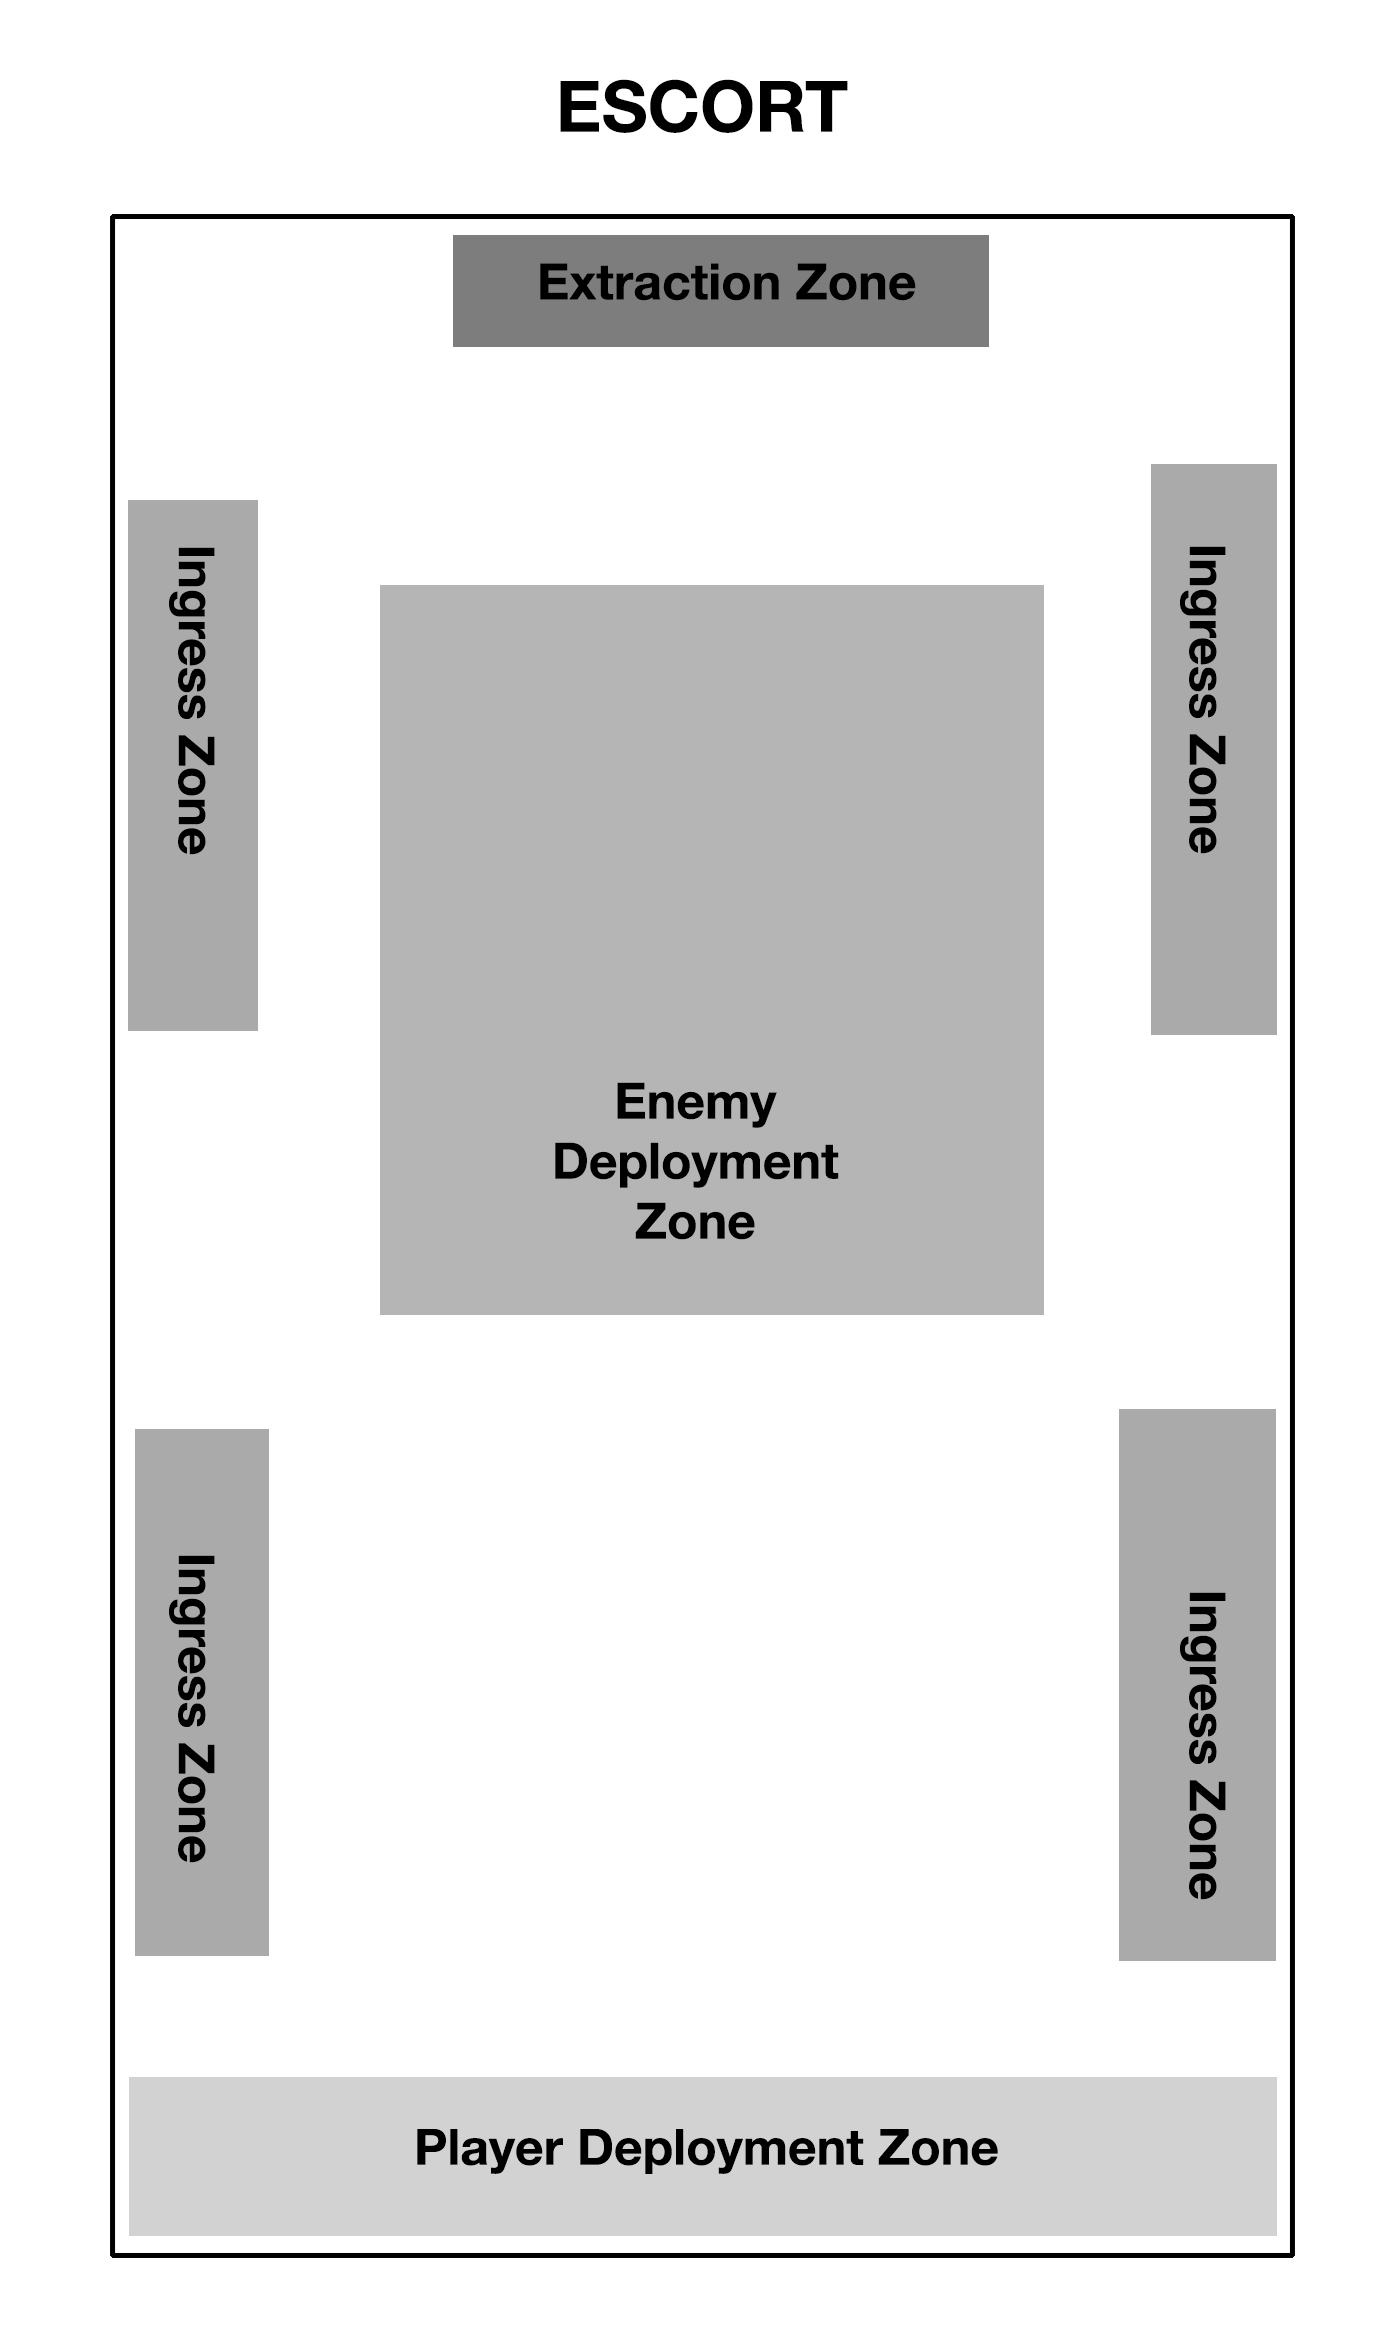
\includegraphics[width=0.50\textwidth]{Sitrep-Escort}
 \end{wrapfigure}
 ``Listen up, Administrator: when we open these doors, you need to stay with us, and you need to do exactly what we tell you to do. If I go down, don't help me -- listen to Monk. If Monk gets hit, listen to Cross. If Cross gets hit, listen to Crown. If Crown dies, keep running and don't stop, and remember: if you make it out of the city, we win the war. Ready?'' -Archived audio, Captain Pyotr ``Pat'' Malov, Cornucopian Revolutionary Guard (KIA)

 An \textbf{ESCORT} mission requires bringing an \textbf{Objective} safely to the Extraction Zone and extracting all player characters safely.

 \textbf{Objective:} The Objective is a size 1/2 - size 2 object, person, or NPC. It has 10 HP/size, evasion 10, e-defense 10, and no armor. The enemy forces want the objective and will not willingly damage it. If any actor starts adjacent to the Objective, they can move the objective with them when they make their regular move on their turn, maintaining adjacency. If the objective is adjacent or becomes adjacent to two actors of opposing sides, it immediately stops moving and can't move until there is only one side in adjacency to it. Otherwise it does not move on its own.

 \textbf{Enemy Forces:} The GM should hold about 2x the enemy forces for a normal encounter. They can deploy up to 1x initially and hold the rest in reserve.

 \textbf{Deployment:} The players deploy first, placing both their characters and the Objective in the deployment zone, then the GM deploys in the enemy deployment zone.


 \textbf{Reserves:} The GM can bring in 1 NPC (or up to 4 grunts) at the start of any new round in one of the Ingress Zones. They cannot choose the same zone twice in a row.

 \textbf{Extraction:} Any player character can extract as a free action at the end of their turn while in the extraction zone. This removes them from the battlefield (they have gotten away safely). If they extract with the objective adjacent to them and no other actor is contesting it, they take the objective with them.

 \textbf{Victory conditions:}
 - The players win if they extract the objective.
 - At the end of the 6th round, if the objective hasn't been extracted, the enemy forces win. If any players are left on the battlefield after the 6th round ends, they are captured or overrun.
 - Nobody wins if the objective is destroyed. The players must still extract to leave safely.
 \newpage
 \subsection{Control}

 ``Take the hill.'' - Common final order

 \begin{figure}\begin{center}
   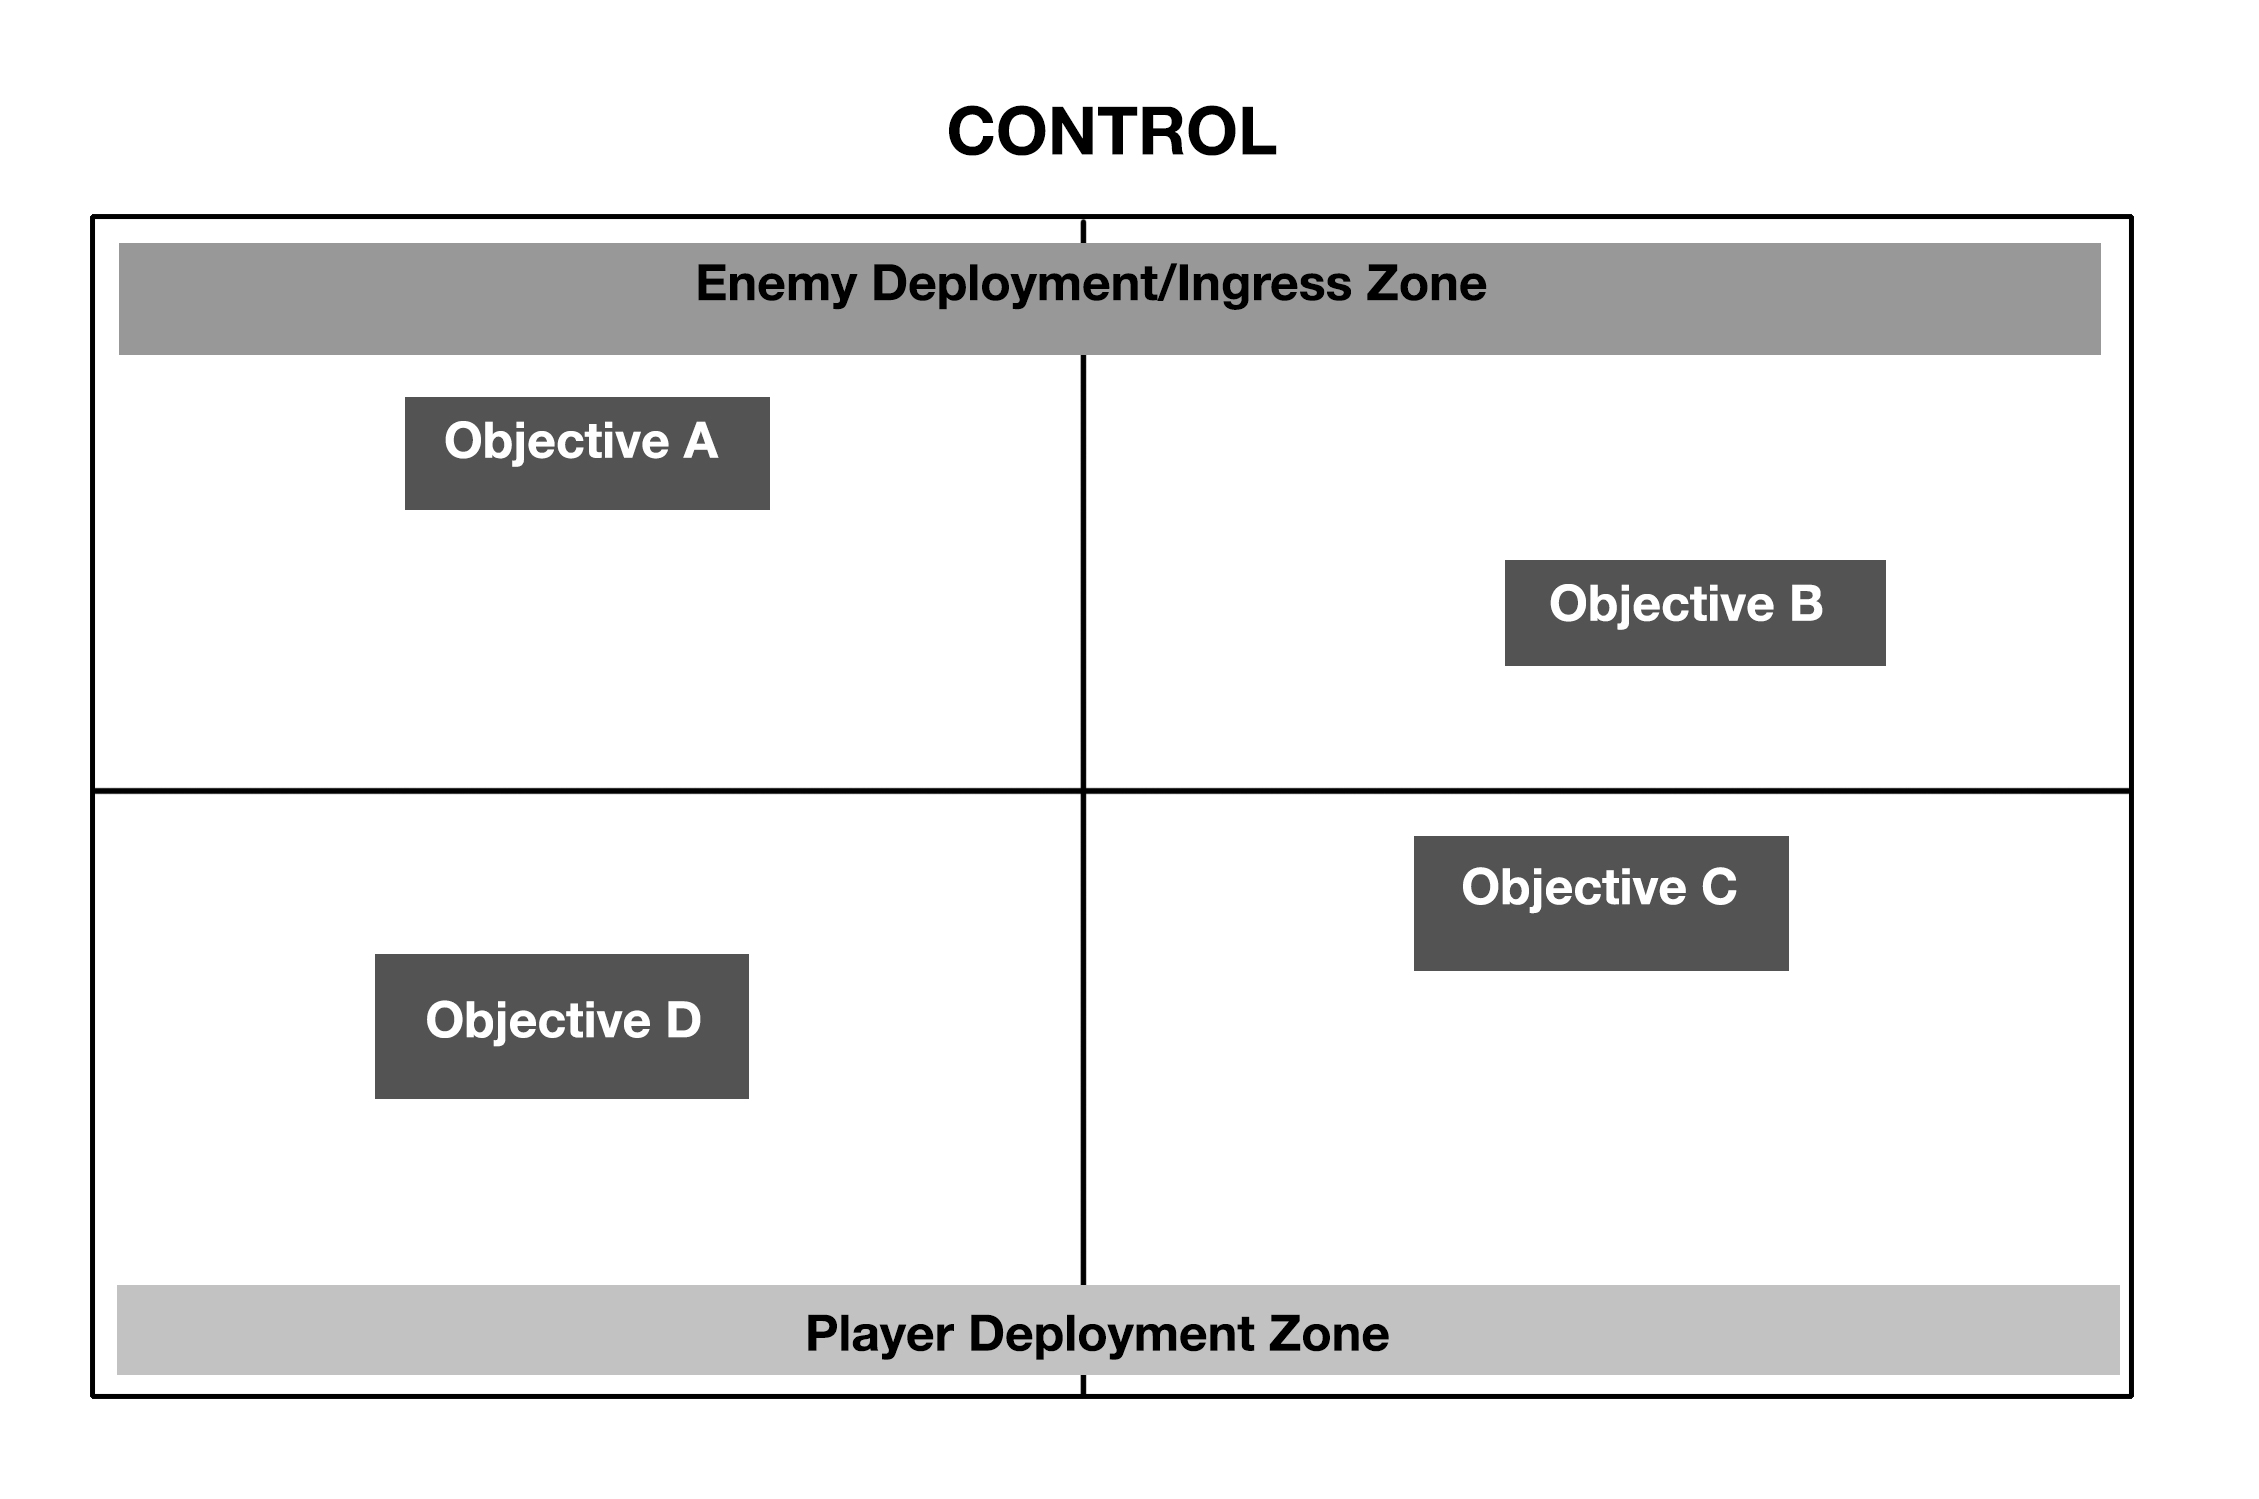
\includegraphics{Sitrep-Control}
 \end{center}\end{figure}

 A \textbf{CONTROL} mission requires maintaining control of four objective zones for six rounds. The zones could be important mission points like transmission towers or gun batteries, terminals or hangars.

 \textbf{Objectives:} There are 4 objective zones (by default you can use roughly 4x4 areas), each placed anywhere in one quadrant of the map. If they are not roughly symmetrical, the map will be unbalanced.

 \textbf{Deployment:} Roll off (1d6) between the players and enemy forces. The loser deploys first in their appropriate zone. The GM can hold enemy forces in reserve if they want but doesn't have more than normal available.

 \textbf{Zone control:} If only actors of one side are inside a zone, they control that zone. If there are actors from two or more sides inside a zone, the zone is contested.

 \textbf{Objective Scoring:} At the end of each round, for each zone a side controls, give them 1 point. If they control all four zones, give them a bonus +1 point.

 \textbf{Victory conditions:} The side with the highest score at the end of round 6 wins.

 \newpage
 \subsection{Extract}

 \begin{wrapfigure}{l}{0.50\textwidth}
   \centering
   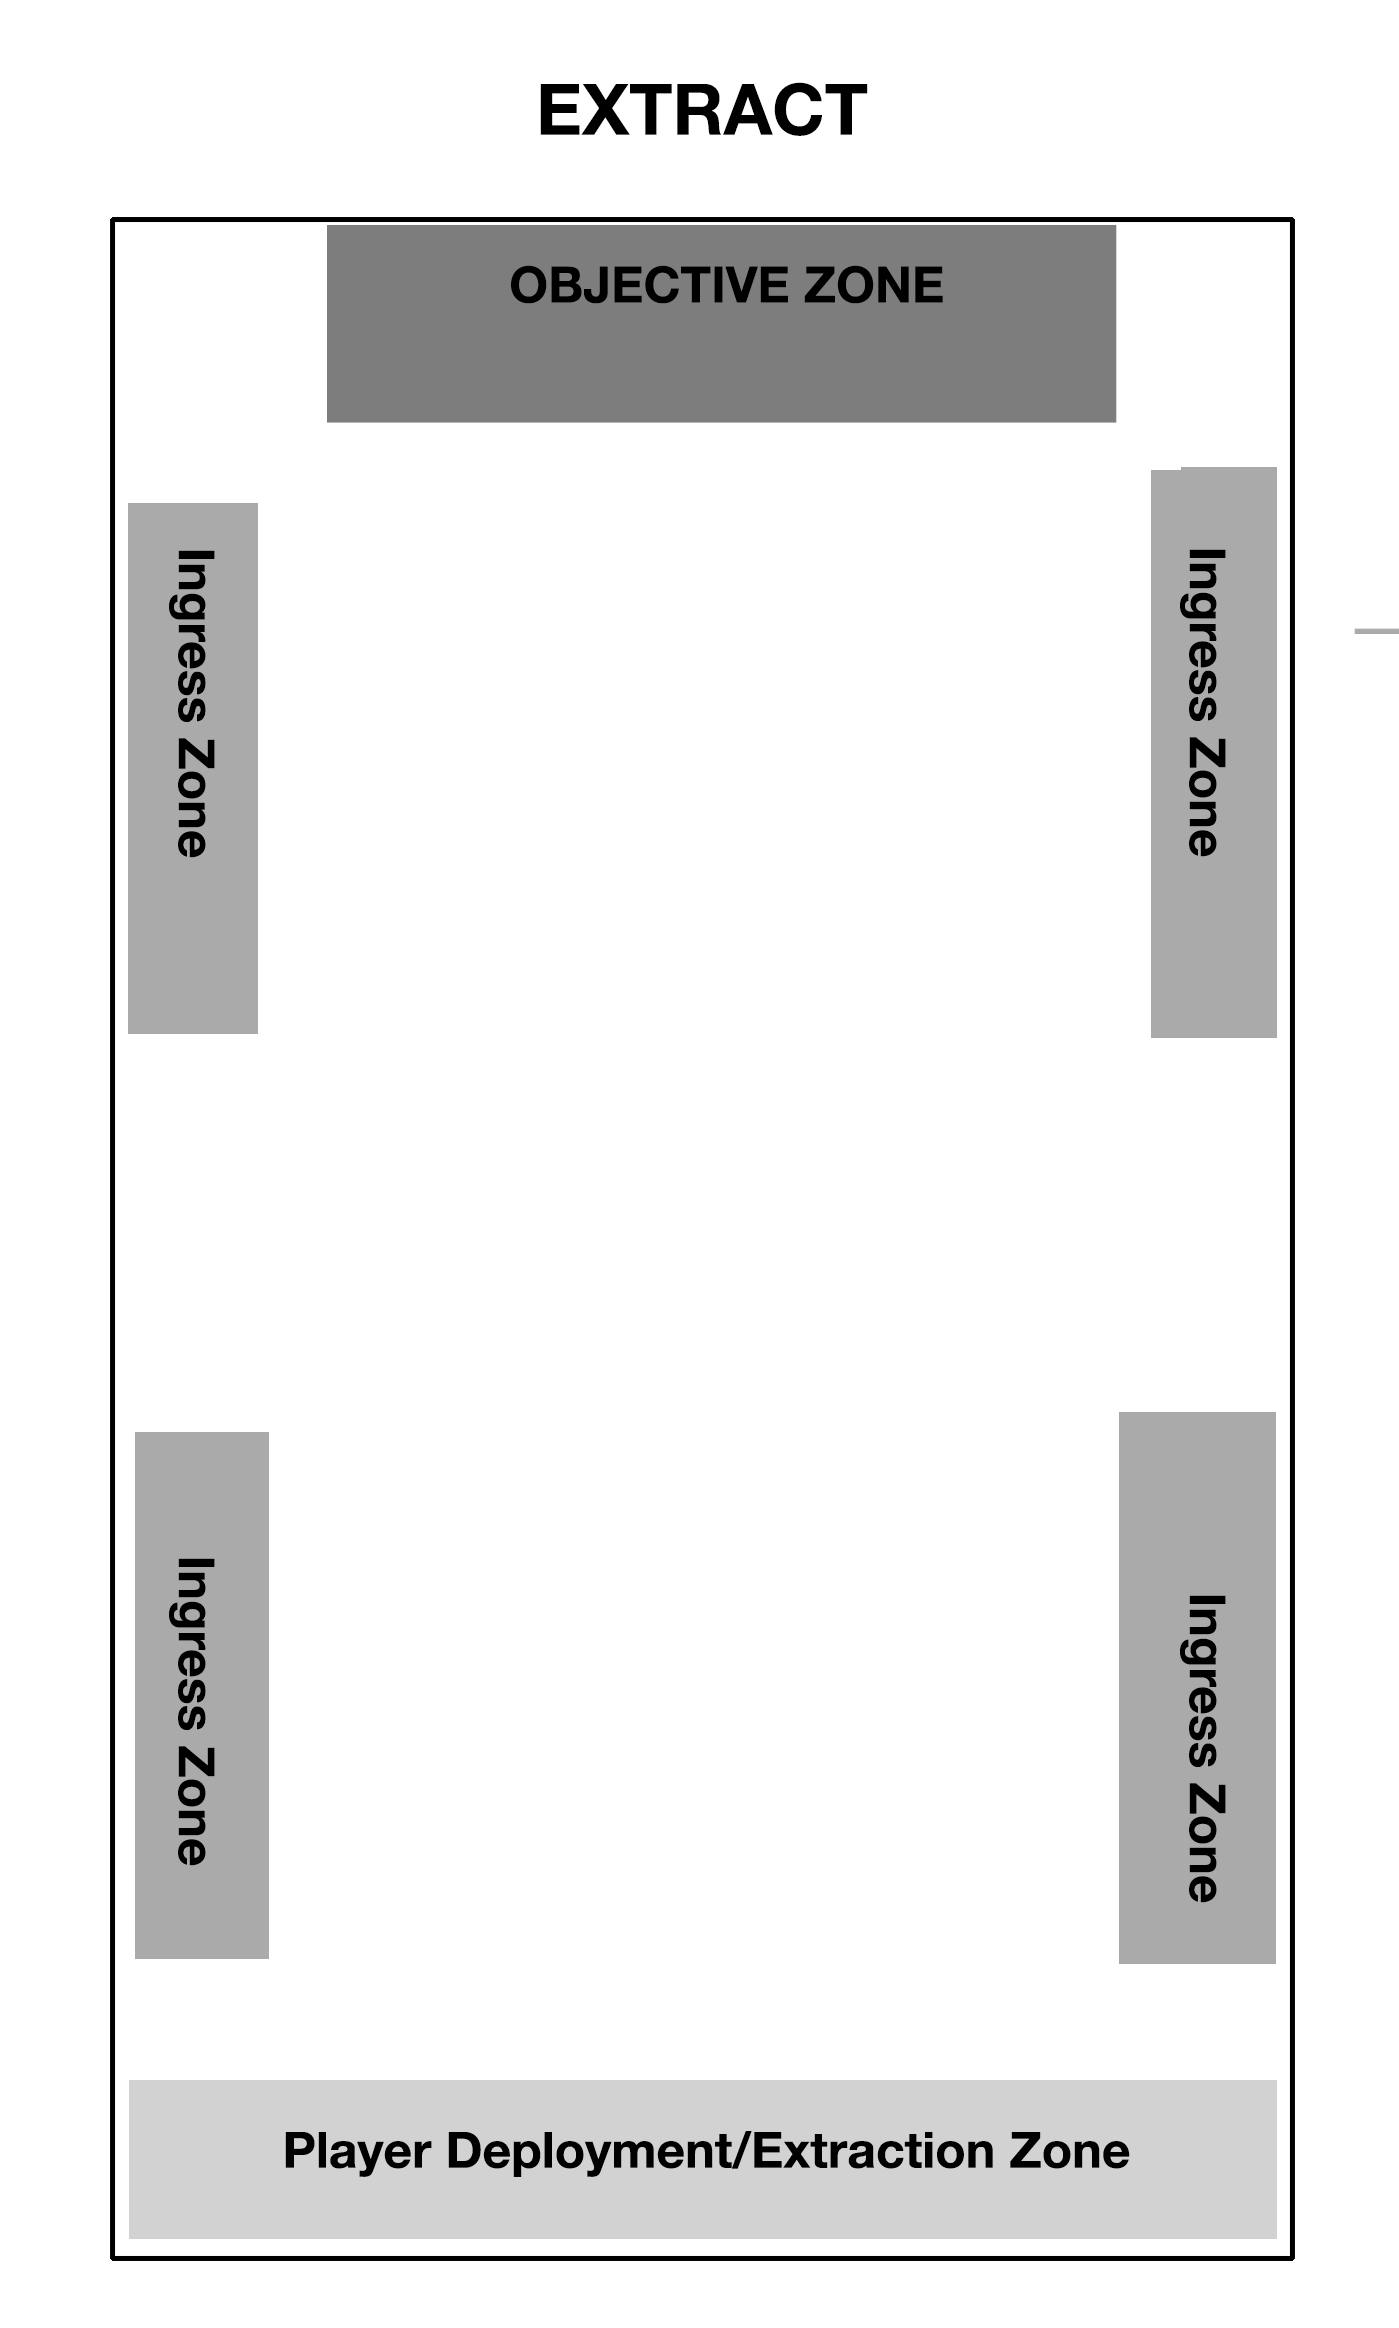
\includegraphics[width=0.50\textwidth]{Sitrep-Extract}
 \end{wrapfigure}

``Catapult Actual, this is Catapult-2: requesting immediate evac from current GRIDCOR'' ``Cat-2 confirm GRIDCOR.'' ``Confirming… Confirmed, Catapult Actual. Air-ground clear and holding. We, uh, have multiple down. KIA and wounded.'' ``Heard, Cat-2. Lifeflight on the way. Confirm: VIP secure.'' ``VIP --'' ``Say again Cat-2.'' ``VIP secure -- We've got more company down here, Actual -- going dark, respond to GRIDCOR.'' ``Confirmed, 2. We're on our way,

An extraction mission is similar to an escort mission, though different in a couple of key areas.

\textbf{Objective:} The Objective is a size 1/2 - size 2 object, person, or NPC. It has 10 HP/size, evasion 10, e-defense 10, and no armor. The enemy forces want the objective and will not willingly damage it. If any actor starts adjacent to the Objective, they can move the objective with them when they make their regular move on their turn, maintaining adjacency. If the objective is adjacent or becomes adjacent to two actors of opposing sides, it immediately stops moving and can't move until there is only one side in adjacency to it. Otherwise it does not move on its own.

\textbf{Enemy Forces:} The GM should hold about 2x the enemy forces for a normal encounter. They hold them all in reserve (round 1 there will be no enemy forces).

\textbf{Deployment:} The players deploy first, placing their characters in the deployment zone. The GM places the Objective in the objective zone.

\textbf{Reserves:} The GM can bring in 2 NPCs (or up to 4 grunts) at the start of any new round in two of the Ingress Zones.

\textbf{Extraction:} Any player character can extract as a free action at the end of their turn while in the extraction zone, which is the same as the deployment zone. This removes them from the battlefield (they have gotten away safely). If they extract with the objective adjacent to them and no other actor is contesting it, they take the objective with them.

\textbf{Victory conditions:} - The players win if they extract the objective. - At the end of the 8th round, if the objective hasn't been extracted, the enemy forces win. If any players are left on the battlefield after the 8th round ends, they are captured or overrun.


 \newpage
 \subsection{Holdout}

 MJ sat in his open cockpit, chewed his gum, and ignored the briefing. Was for the local Oxes, kids and eagers who needed a pep talk, not him and his Emancipators. They got the real story. Real story wasn't a pretty pic. Extract was six hours out and burning hard. The Crown horse guards got a hundred mix 'n match middle-tier Armory shells, couple thou' cavalry -- poor damn horses. MJ had a thousand rounds of hardpoint EX, two racks of Kodandams, and his MC-TB for when the real mess came. ``Yo MJ,'' his comms squawked. ``Button up. We got company, four hundred meters out and closing. Horses.'' ``Uh huh,'' MJ said. He slapped the cabin seal without looking and got comfortable. Helm on, haptics on. Mag loaded. Feel bad for the horses, because they didn't know what they were getting into. Six hours to extract, clock starting now.

 \begin{figure}\begin{center}
   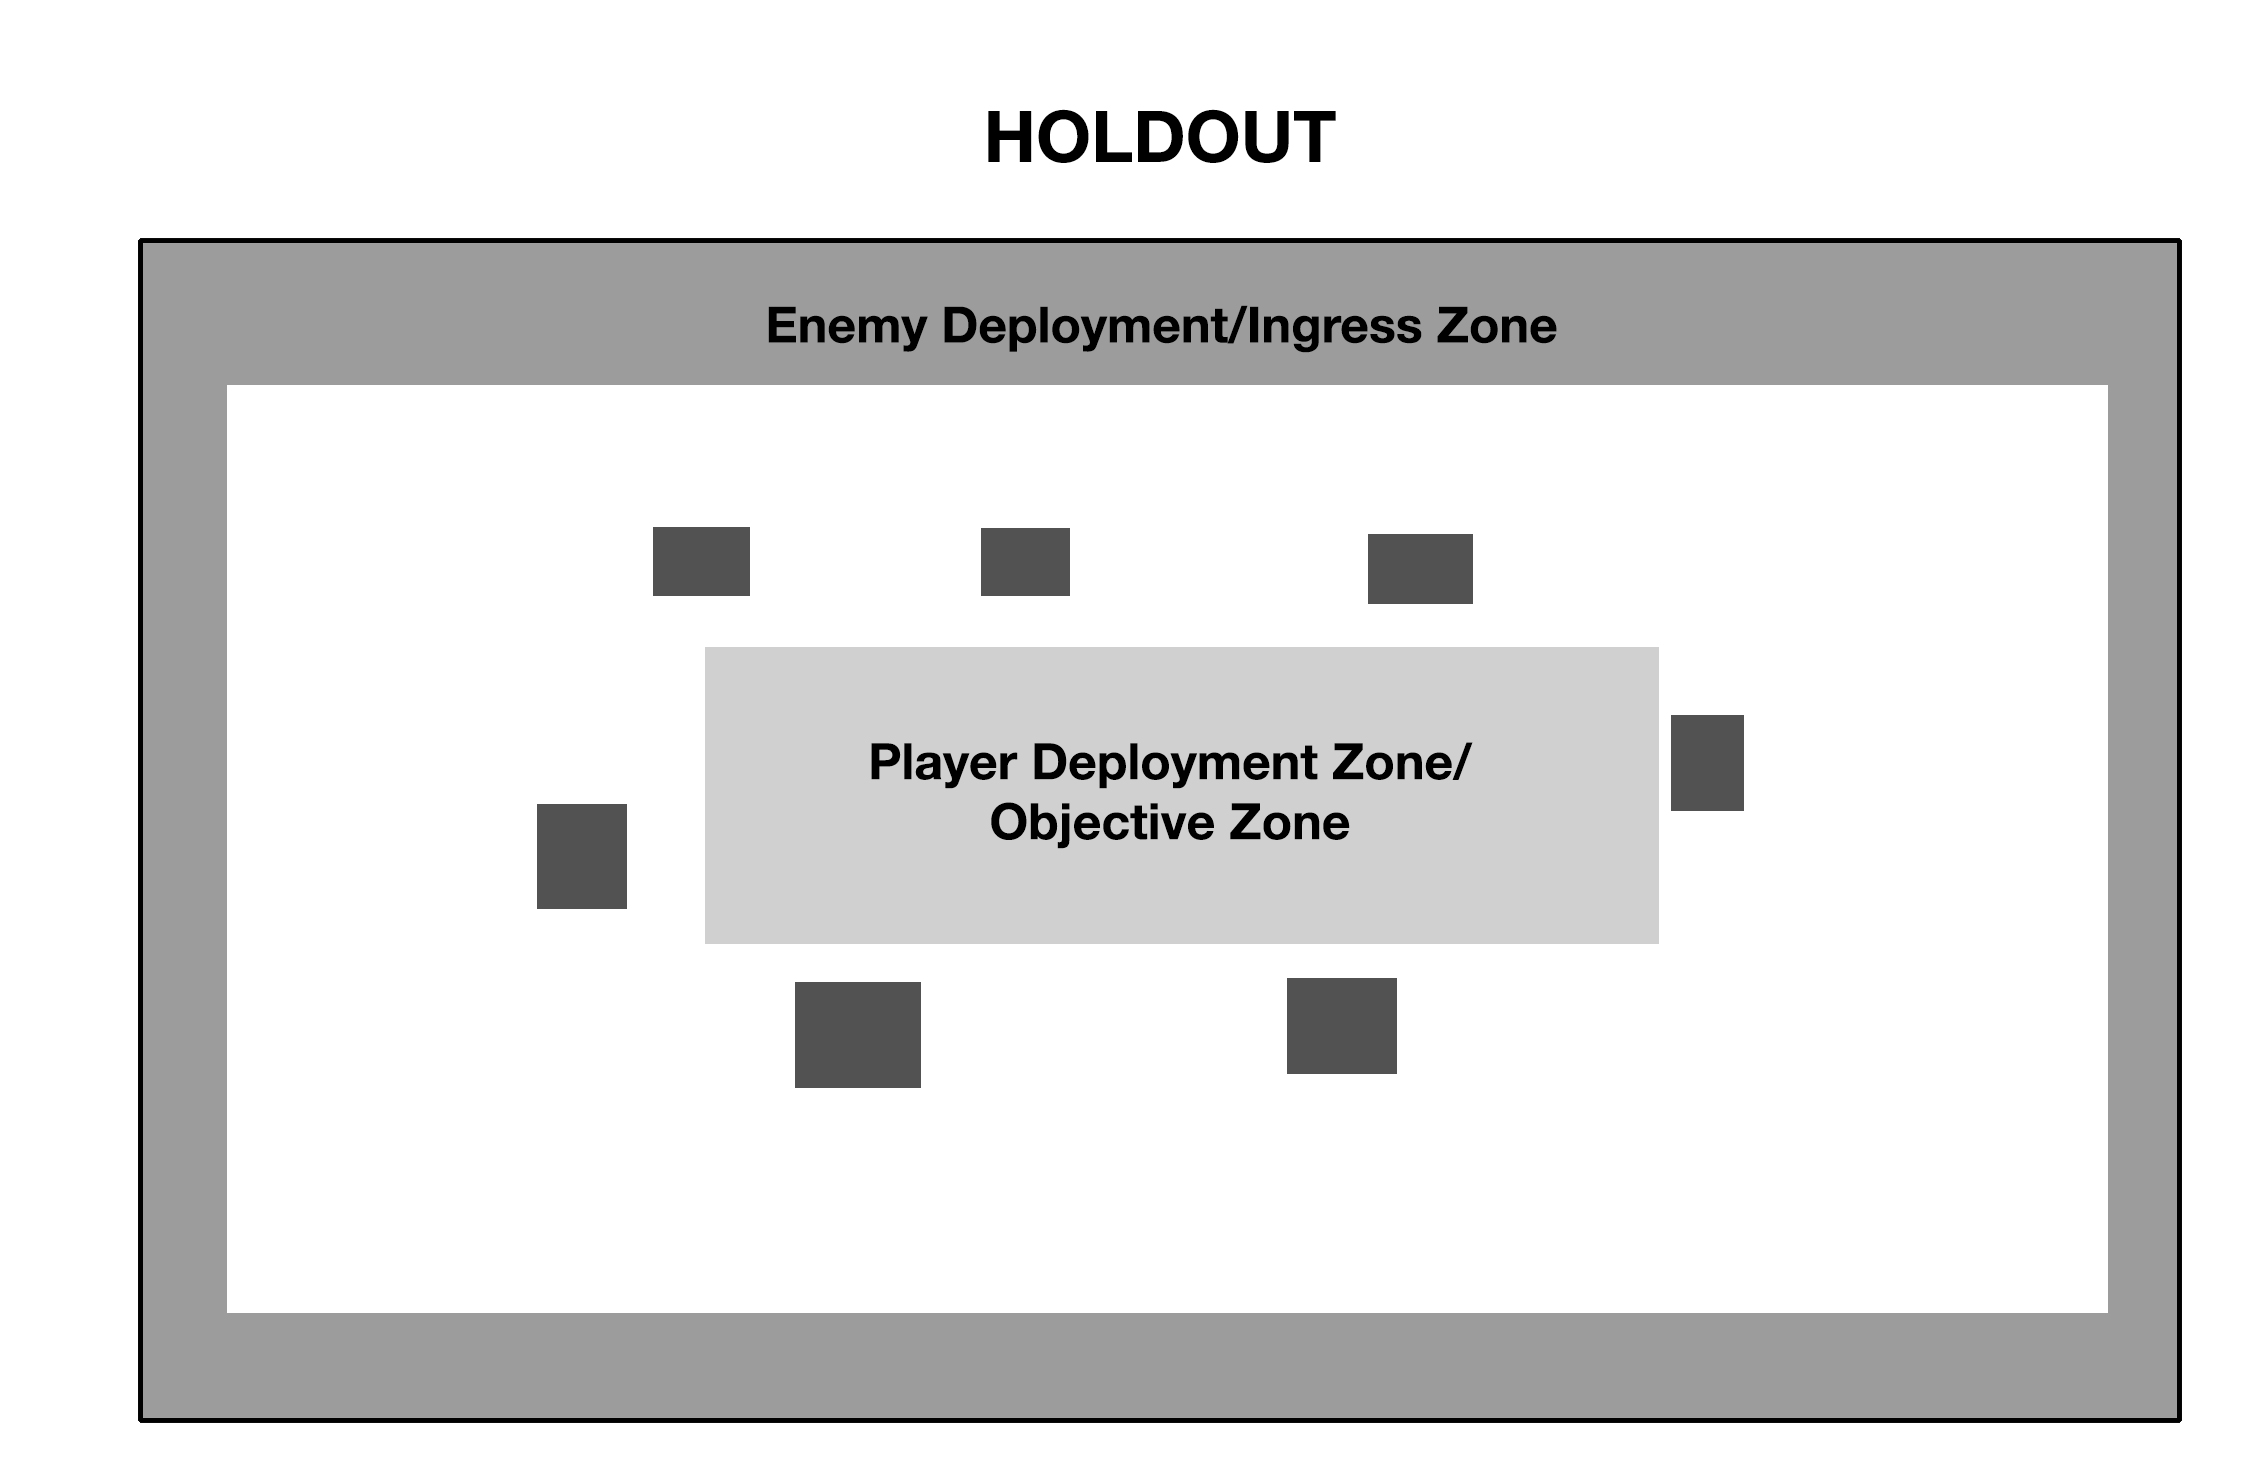
\includegraphics{Sitrep-Holdout}
 \end{center}\end{figure}

 A desperate mission type. When ordered to Hold Out, players will have to defend an area against an onslaught of enemies -- in a best-case scenario, this is to buy time for allies to complete an objective elsewhere. In a worst-case scenario, it is to the death.

 \textbf{Enemy Forces:} The GM should hold about 2x the enemy forces for a normal encounter. They hold half in reserve

 \textbf{Deployment:} The players deploy first, then the GM deploys half their total forces.

 \textbf{Fortifications:} The area around the objective zone should have size 1-2 heavy cover

 \textbf{Objective:} The objective zone is a roughly 10 spaces by 5 spaces area in the middle of the map (you can adjust this as needed). Players start with 4 points. For every enemy inside of the objective zone, the players get -1 points (the score could go negative).

 \textbf{Victory conditions:}  If at the end of round 6 the player characters are alive and their score is 1 or greater, they win, otherwise they are captured or overrun.


 \newpage
 \subsection{Gauntlet}

 \begin{wrapfigure}{l}{0.50\textwidth}
   \centering
   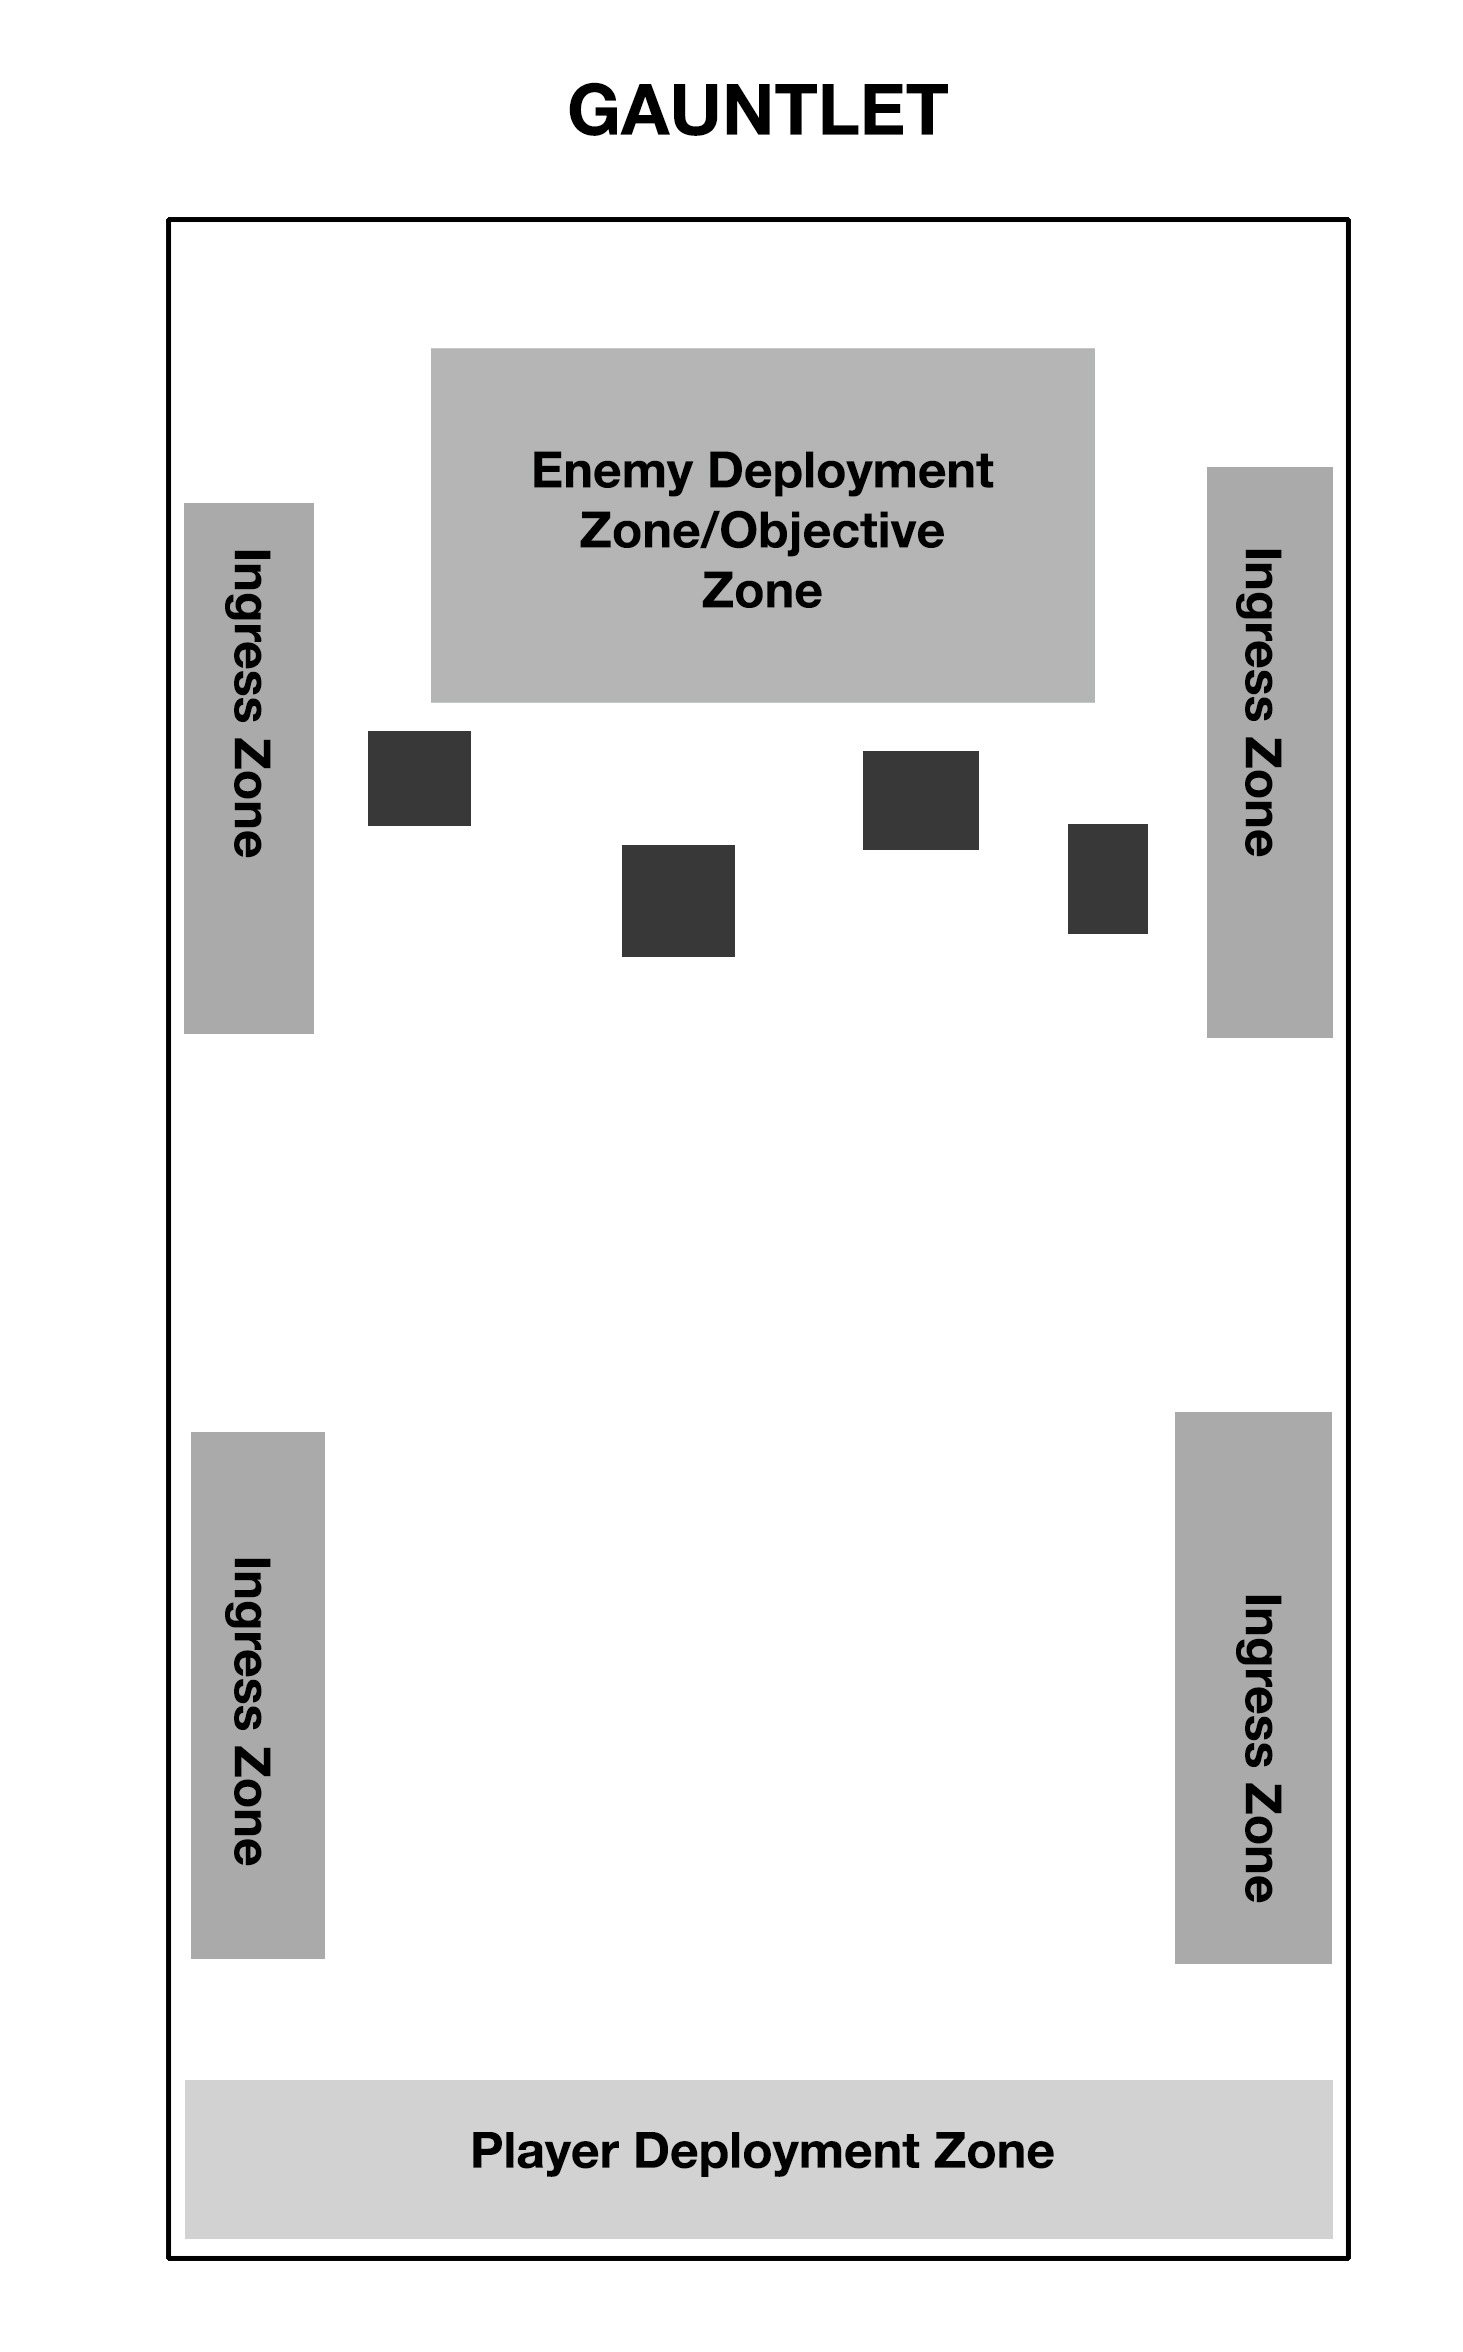
\includegraphics[width=0.50\textwidth]{Sitrep-Gauntlet}
 \end{wrapfigure}

>// [WHITEOUT CONTINGENCY:: REAR ECHELON HAS FALLEN. ALL UNITS AT
MINIMUM/NEGATIVE EFFICACY]

>//[ALL-BAND ORDER::PROCEED AT TOTAL STRIKE CAPACITY TO ID EXTRACT AREA]

>//[THIS IS A IMPERATIVE COMPLY ORDER. YOU ARE ON YOUR OWN++OUR POSITION IS
OVERRUN++HURRY]

Generally a mission done under duress, or when no other options are available to the players. Commonly engaged in unfriendly terrain. A Gauntlet mission demands the player party move from their deployment zone across unfriendly territory to secure an enemy position.

\textbf{Enemy forces:} The GM should have a normal amount of enemy forces, but hold half in reserve.

\textbf{Deployment:} The GM deploys half their forces first, then the players deploy

\textbf{Fortifications:} The area around the enemy deployment zone is fortified with size 1 and 2 heavy cover

\textbf{Reserves:} At the end of round 1, the GM deploys the rest of their forces in any of the Ingress zones

\textbf{Victory conditions:} The players win if there are more player characters inside the objective zone at the end of turn 6 than enemy characters (count ultras for 4 players, elites for 2, and grunts for 1/4). Otherwise the enemies win.

 \newpage
 \subsection{Recon}
 Aurelia whistled low, taking in the fresh coat of matte on their chassis. ``Optical camo overlay primary, Inkwell secondary,'' Engineer Coates said, finishing her walkaround. ``Even if they scramble your anoptics, it's going to be a nightmare to sight her.'' Aurelia reached up to touch their chassis' brachial mount. Their sylph spilled across their arm, touched the chassis. An inkbloom of the midnight color clouded through it. Aurelia grinned. They would be a nightmare.

 \begin{center}
   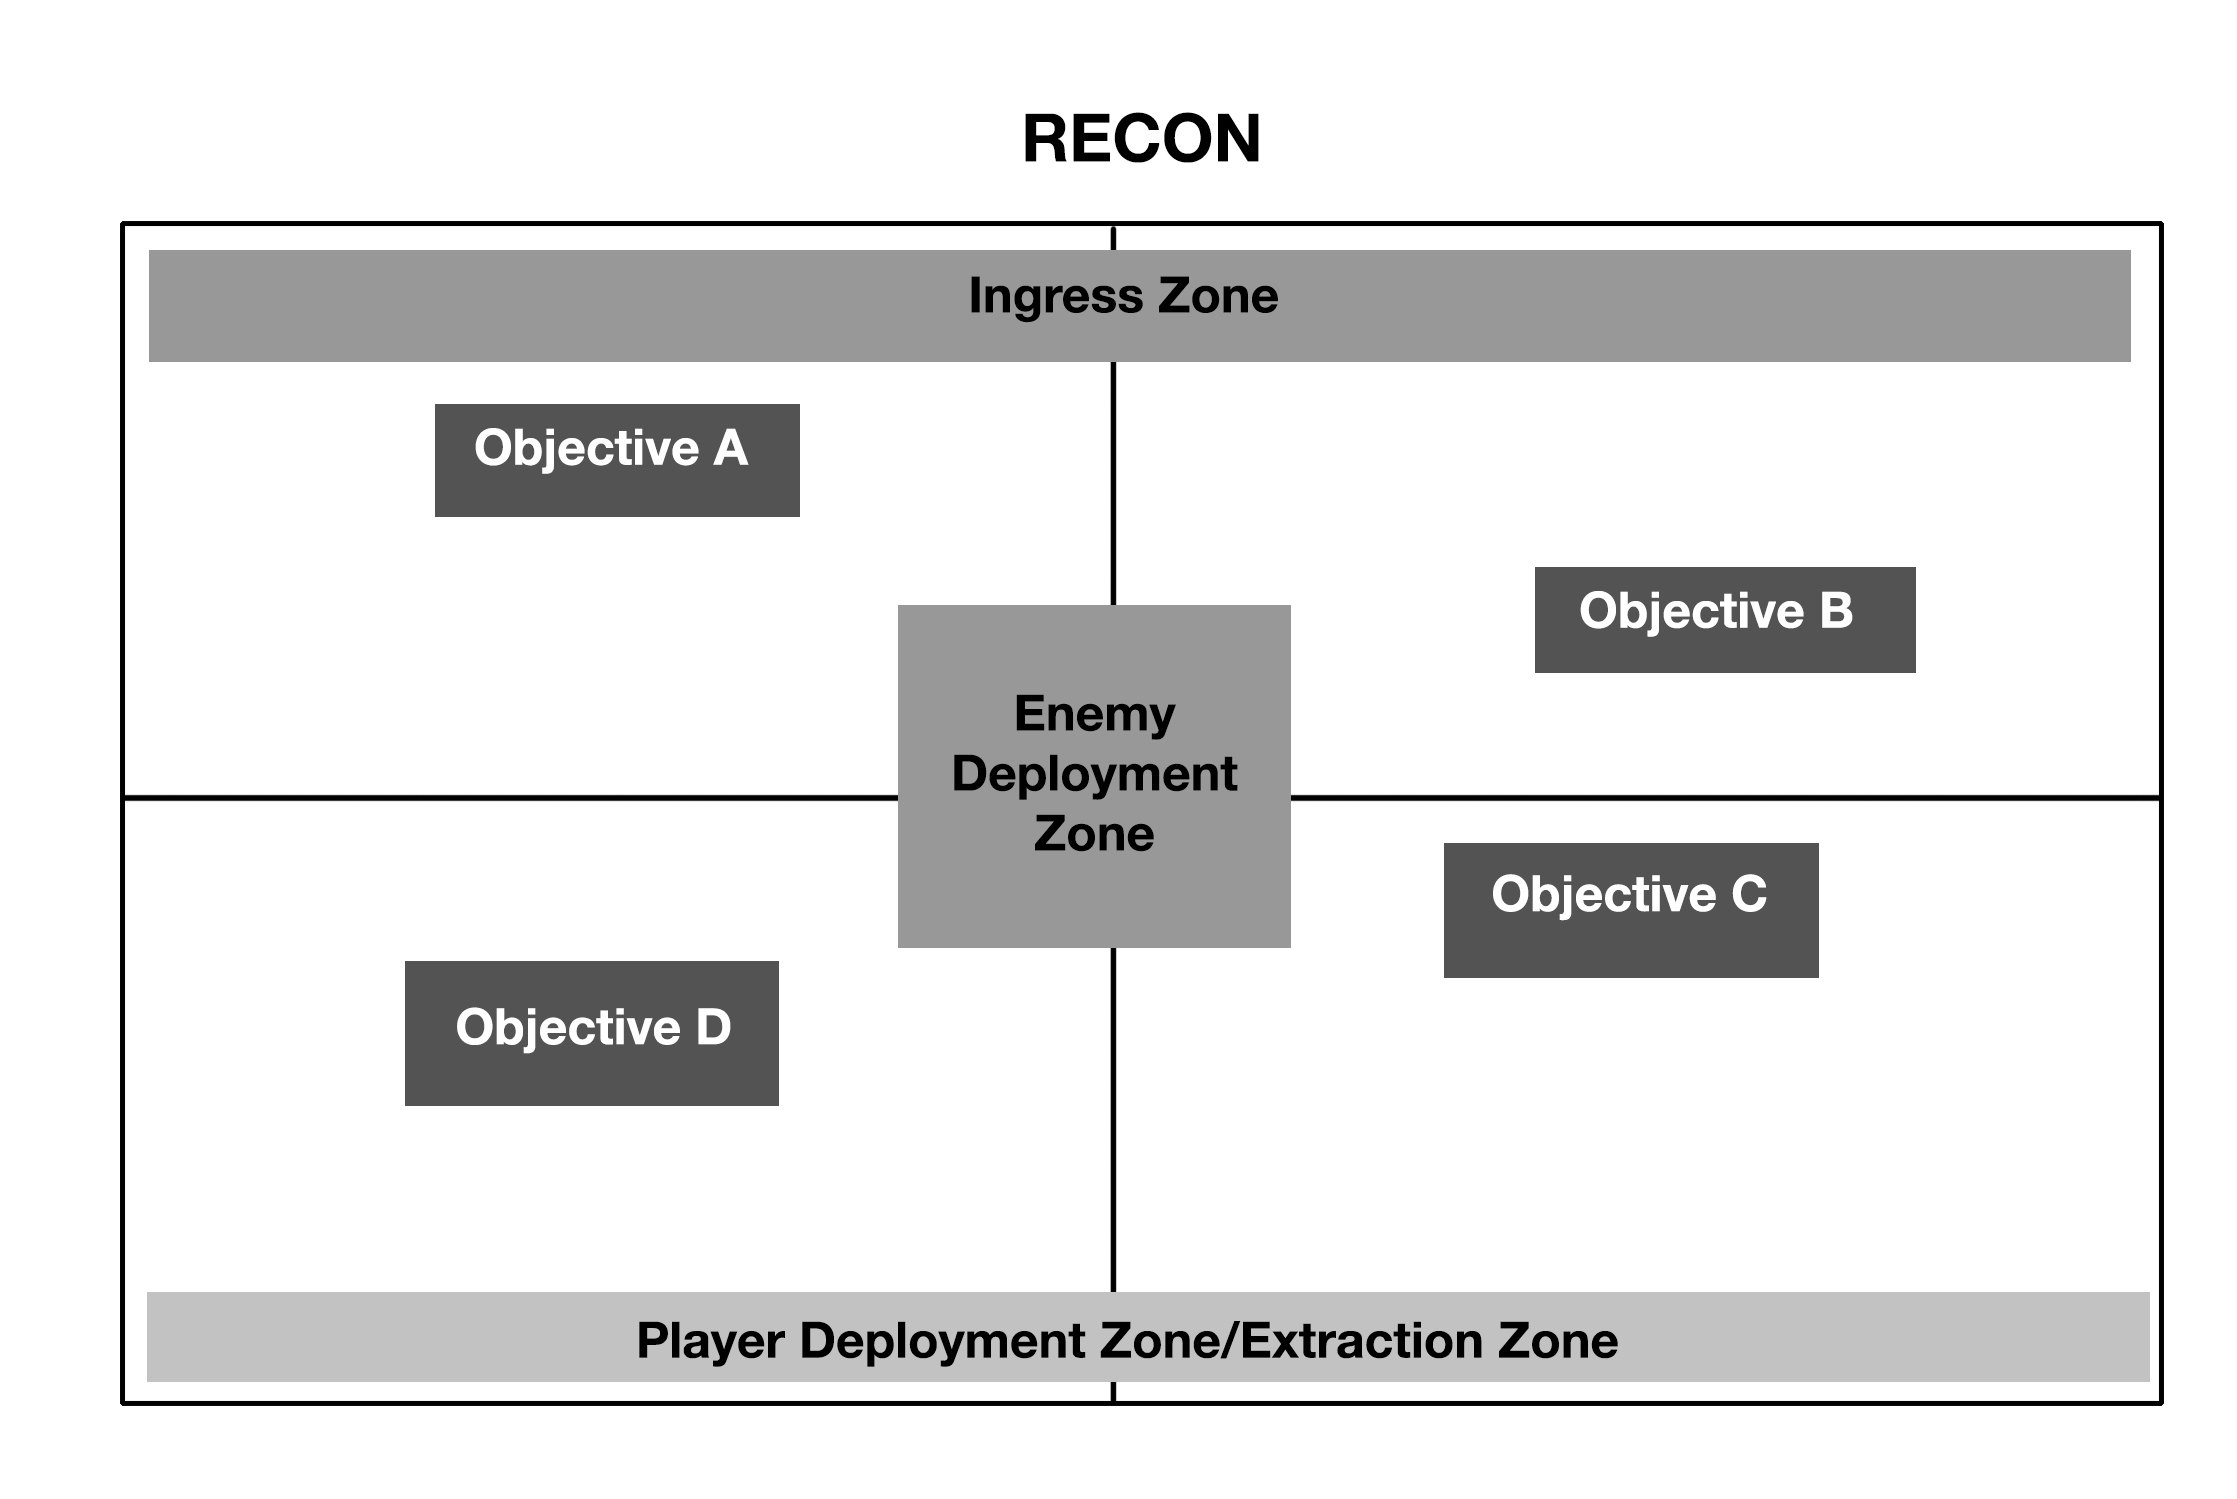
\includegraphics{Sitrep-Recon}
 \end{center}

 A recon mission is, generally speaking, a dangerous endeavor, where a small team enters hostile territory to identify targets or retrieve key information

 \textbf{Objectives:} The GM marks 4 4x4 objective zones on the map. The GM secretly chooses one of the objectives to be the real objective (from A-D). Characters can control an objective by being the only side inside the objective zone at the end of the round. They can determine whether the objective is real or not by being inside the zone and taking a full action (this information is freely shareable once discovered). They don't need to control the zone to investigate it.

 \textbf{Enemy Forces:} The GM has normal enemy forces, and can hold any number in reserve

 \textbf{Deployment:} The players deploy first, then the NPCs

 \textbf{Reserves:} The GM can bring in 1 NPC or up to 4 grunts in the ingress zone at the start of any new round.

 \textbf{Victory conditions:} The players win if they are in control of the real objective at the end of round 6. Otherwise, the enemy forces win.
